\documentclass[12pt,bahasa]{article}
\usepackage[a4paper]{geometry}
\geometry{verbose,tmargin=1.5cm,bmargin=1.5cm,lmargin=1.5cm,rmargin=1.5cm}
\usepackage{amsmath}
    
\setlength{\parindent}{0cm}
  
\usepackage{float}
\usepackage{graphicx}
\usepackage{enumitem}
\usepackage{hyperref}
\usepackage{url}
\usepackage{xcolor}
\usepackage{babel}

\usepackage{minted}
\newminted{scilab}{breaklines}

\definecolor{mintedbg}{rgb}{0.95,0.95,0.95}
\usepackage{mdframed}

\BeforeBeginEnvironment{minted}{\begin{mdframed}[backgroundcolor=mintedbg]}
\AfterEndEnvironment{minted}{\end{mdframed}}

\begin{document}

\title{Tugas Besar TF2202}
\date{}
\maketitle

%\begin{scilabcode}
%function [a,b] = func1(c,d)
%  // Test comment
%endfunction
%\end{scilabcode}

Selesaikan soal-soal berikut ini dengan menggunakan Scilab.

%=====================================================
\section{Perbandingan akurasi beberapa metode untuk ODE}
%=====================================================

Carilah solusi numerik dari persamaan diferensial berikut
\begin{equation}
y''(t) + y(t) = 0
\end{equation}
dengan syarat awal
\begin{equation}
y(0) = 0, \hspace{0.5cm} y'(0) = 1
\end{equation}
pada interval $0 \leq t \leq 10$.

Bandingkan solusi yang diperoleh dengan solusi analitik:
\begin{equation}
y(t) = \sin(t)
\end{equation}

Gunakan menggunakan metode-metode berikut ini untuk mencari solusi numeriknya.
\begin{itemize}
\item Euler
\item Euler dengan prediktor-korektor (Runge-Kutta orde-2)
\item Runge-Kutta orde-4
\end{itemize}

Dari solusi numerik yang didapatkan, buatlah (1) plot antara $y$ dan $y'$
dan (2) plot antara $t$ dan $y$.

%=================================
\section{Gerakan pendulum}
%=================================

Gerak suatu pendulum dapat dinyatakan dengan persamaan diferensial:
\begin{equation}
\theta''(t) = -\frac{g}{L}\sin(\theta(t)) - k\theta'(t)
\end{equation}
dengan syarat awal
\begin{equation}
\theta(0) = \theta_0, \hspace{0.5cm} \theta'(0) = 0
\end{equation}

\begin{figure}[H]
\centering
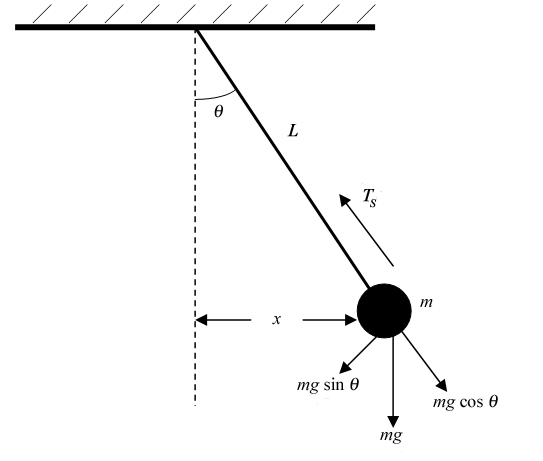
\includegraphics[scale=0.4]{images/pendulum.png}
\par
\caption{Pendulum sederhana}
\end{figure}

Dalam persamaan tersebut $\theta$ menyatakan simpangan pendulum,
$\theta_0$ menyatakan simpangan awal pendulum,
$g$ menyatakan percepatan gravitasi, $L$ menyatakan panjang benang pendulum,
dan $k\theta'$ menyatakan suku redaman (gesekan) yang berbanding lurus
dengan kecepatan $\theta'$ ($k$ adalah bilangan positif).

\begin{enumerate}[label=(\alph*)]
\item Cari solusi $\theta(t)$ untuk kasus $k=0$ untuk simpangan awal $\theta_0 = 0.1, \pi/5$
dan 3.0.
\item Masih untuk kasus $k=0$, tentukan periode osilasi $T$ sebagai
fungsi dari simpangan awal $u_0$.
\item Carilah solusi $u(t)$ untuk kasus $k = 0.1, 0.3, 0.5$ dan 0.8 untuk
simpangan awal yang sama.
\end{enumerate}


%========================================================
\section{Persamaan Schrodinger (metode shooting)}
%========================================================

Persamaan Schrodinger independen-waktu pada 1 dimensi
dapat dinyatakan sebagai berikut.
\begin{equation}
-\frac{\hbar^2}{2m}\frac{\mathrm{d}\psi}{\mathrm{d}x^2}
+ V(x)\psi(x) = E\psi(x)
\label{eq:sch1d}
\end{equation}
Dengan menggunakan unit atomik, kita dapat mengambil $\hbar = 1$
dan $m = 1$, dan persamaan \eqref{eq:sch1d} dapat ditulis menjadi:
\begin{equation}
\psi'' = 2\left[ V(x) - E \right]\psi
\label{eq:sch1d_2}
\end{equation}
Untuk solusi keadaan terikat (bound states), nilai $E$ hanya dapat memiliki
nilai yang diskrit. Selain itu, untuk bound states
fungsi gelombang dibatasi dengan syarat
\begin{equation}
\lim_{x\rightarrow\infty} \psi(x) = 0,\hspace{0.5cm}\lim_{x\rightarrow-\infty} \psi(x) = 0
\end{equation}
Selain itu, fungsi gelombang biasanya juga dinyatakan dalam bentuk ternormalisasi:
\begin{equation}
\int_{-\infty}^{\infty} \psi^{*}(x) \psi(x)\,\mathrm{d}x = 1
\end{equation}

Untuk potensial yang simetrik terhadap $x=0$, secara matematis dapat ditulis
$V(-x) = V(x)$. Contoh potential simetrik yang akan dibahas adalah potensial harmonik
\begin{equation}
V(x) = \frac{1}{2}x^2
\end{equation}
Dengan demikian, kita bisa mendapatkan solusi pada $(-\infty,\infty)$ hanya dengan
solusi pada $(0,\infty)$.
Ingat lagi dari kuliah mekanika kuantum bahwa,
untuk potensial harmonik, nilai $E$ yang diperbolehkan adalah:
\begin{equation}
E = \frac{(n + 1)}{2}, \hspace{0.5cm} n = 0,1,2,\ldots
\end{equation}
Kita dapat mengelompokkan solusi ini menjadi dua kelompok:
\begin{itemize}
\item solusi ganjil ($n = 1, 3, 5, \ldots$), dengan fungsi gelombang
$\psi(x) = -\psi(-x)$
\item solusi genap ($n = 0, 2, 4, \ldots$), dengan fungsi gelombang
$\psi(x) = \psi(-x)$
\end{itemize}

Persamaan \eqref{eq:sch1d_2} dapat diselesaikan dengan
menggunakan metode standard seperti Runge-Kutta
orde-4. Metode lain yang sering digunakan adalah metode Numerov. Metode ini biasa
digunakan untuk menyelesaikan persamaan diferensial orde dua tanpa suku dengan turunan
pertama, seperti pada persamaan \eqref{eq:sch1d_2}.
Metode ini dapat dituliskan dalam bentuk:
\begin{align}
u_{m} & = 1 - \dfrac{1}{6}h^2 \left[ V(x_m) - E \right] \\
\psi_{m+1} & = \dfrac{\left(12 - 10u_{m}\right)\psi_{m} - u_{m-1}\psi_{m-1}}{u_{m+1}}
\end{align}

Untuk mengaplikasikan metode shooting, persamaan nilai batas harus dikonversi menjadi
permasalahan syarat awal:
\begin{align}
\psi(0) & = \psi_{0},\hspace{0.5cm} \psi'(0) = 0,\hspace{0.5cm} n = 0,2,4,\ldots \\
\psi(0) & = 0,\hspace{0.5cm} \psi'(0) = \psi'_{0},\hspace{0.5cm} n = 1,3,5,\ldots
\end{align}
Nilai dari $\psi_0$ dan $\psi'_0$ dapat dipilih dengan nilai sembarang bukan nol.
Untuk soal ini kita akan ambil $\psi_0 = 1$ dan $\psi'_0 = 1$.

\begin{enumerate}[label=(\alph*)]
\item Buatlah program untuk menghitung solusi numerik dari persamaan \ref{eq:sch1d_2}
dengan menggunakan metode Numerov. Perhatikan bahwa untuk mendapatkan nilai $\psi_{m+1}$ kita memerlukan dua nilai
sebelumnya, yaitu $\psi_{m}$ dan $\psi_{m-1}$, sedangkan dari deskripsi masalah kita
biasanya hanya memiliki informasi nilai awal $\psi_{0}$ dan $\psi'_{0}$.
Untuk mencari nilai $\psi_{1}$ kita dapat menggunakan metode Euler-Cromer:
\begin{equation}
\psi_{1} = \psi_{0} + \psi'_{0}\Delta x + 2(V(x_{0}) - E)(\Delta x)^2
\end{equation}
Gunakan nilai solusi analitik $E = 0.5$ dan disekitarnya misalnya $E = 0.499$ dan $0.501$
serta bandingkan hasilnya numerik dari $\psi$ yang didapatkan dengan
$\psi$ eksak, yaitu $\psi = \exp(-x^2/2)$.
Anda dapat mengaproksimasi solusi pada selang $0 \leq x < \infty$
dengan solusi selang $0 < x < 5$, misalnya dengan asumsi bahwa fungsi gelombang
eksak telah memiliki nilai nol pada $x = 5$.
Gunakan juga syarat awal yang sesuai untuk $E = 0.5$ (solusi genap), yaitu
$\psi_{0} = 1$ dan $\psi'_{0} = 0$.
%
\item Gunakan metode shooting dengan cara memvariasikan nilai $E$ untuk mencari
nilai $E$ yang mungkin dalam rentang $0 \leq E \leq 15$. Gunakan syarat awal
yang sesuai untuk solusi ganjil dan genap.
\end{enumerate}


%====================================================
\section{Persamaan Schrodinger (nilai eigen)}
%====================================================

Metode alternatif
yang dapat digunakan untuk menyelesaikan persamaan
Schrodinger independen-waktu adalah dengan menyelesaikan
persamaan eigenvalue
\begin{align}
\left[-\frac{\mathrm{d}^2}{\mathrm{d}x^2} + V(x)\right]\psi(x) & = E\psi(x) \\
\hat{H}\psi(x) & = E \psi(x)
\end{align}
Nilai-nilai $E$ yang mungkin dapat dicari dengan cara menghitung
nilai eigen dari matriks Hamiltonian 
\begin{equation}
H_{ij} = K_{ij} + V_{ij}
\end{equation}
Dengan $K_{ij}$ dan $V_{ij}$ adalah representasi matriks dari operator
kinetik dan potensial.
Fungsi eigen terkait adalah fungsi gelombang solusi dari
persamaan \eqref{eq:sch1d_2}.

Suatu selang $-L < x < L$ dengan $L$ suatu bilangan positif
dibagi-bagi kedalam $N-1$ partisi dengan jumlah total titik $N$,
yaitu $x_{i}$, $i = 1, 2, \ldots, N$.
Potensial $V(x)$ dapat dihitung pada $x_{i}$ sehingga
kita peroleh representasi diskrit dari potensial:
$V_{i} = V_(x_{i})$.

Matriks $V_{ij}$ adalah matriks diagonal yang elemen diagonalnya adalah
nilai dari $V(x)$ pada titik $x_{i}$.

Matriks $K_{ij}$ dapat
dapat diaproksimasi dengan cara mengaproksimasi operator $\mathrm{d}^2/\mathrm{d}x^2$
dengan menggunakan beda hingga.

\begin{enumerate}[label=(\alph*)]
\item Gunakan beda hingga sentral 3 titik untuk mengaproksimasi matriks $K_{ij}$
\item Hitung matriks Hamiltonian dan selesaikan persamaan eigen $H\psi = E\psi$. Anda dapat
menggunakan perintah \texttt{[psi,D] = spec(H); E = diag(D)} pada Scilab.
Bandingkan hasil yang Anda peroleh dengan solusi analitik.
\item Ulangi (a) dan (b) dengan menggunakan beda hingga sentral 5, 7, dan 9 titik.
Bandingkan hasilnya dengan menggunakan $\Delta x$ yang sama.
\end{enumerate}


\section{Persamaan Poisson 2D}

Hitung solusi numerik dari persamaan Laplace:
\begin{equation}
\frac{\partial^2 u(x,y)}{\partial x^2} +
\frac{\partial^2 u(x,y)}{\partial y^2} = \cos(x + y) - \sin(x - y)
\end{equation}
pada domain rektangular $-\pi < x < \pi$, $-\pi < y < \pi$ dengan syarat batas
\begin{equation}
u(\pm\pi,y) = 0, \hspace{0.5cm} u(x,\pm\pi) = 0
\end{equation}
dengan menggunakan metode beda hingga. Gunakan metode Gauss-Seidel untuk
menyelesaikan sistem persamaan linear yang dihasilkan.
Bandingkan solusi numerik yang diperoleh dengan
solusi analitik
\begin{equation}
u(x,y) = \sin(x)\cos(y)
\end{equation}

\begin{figure}[H]
\centering
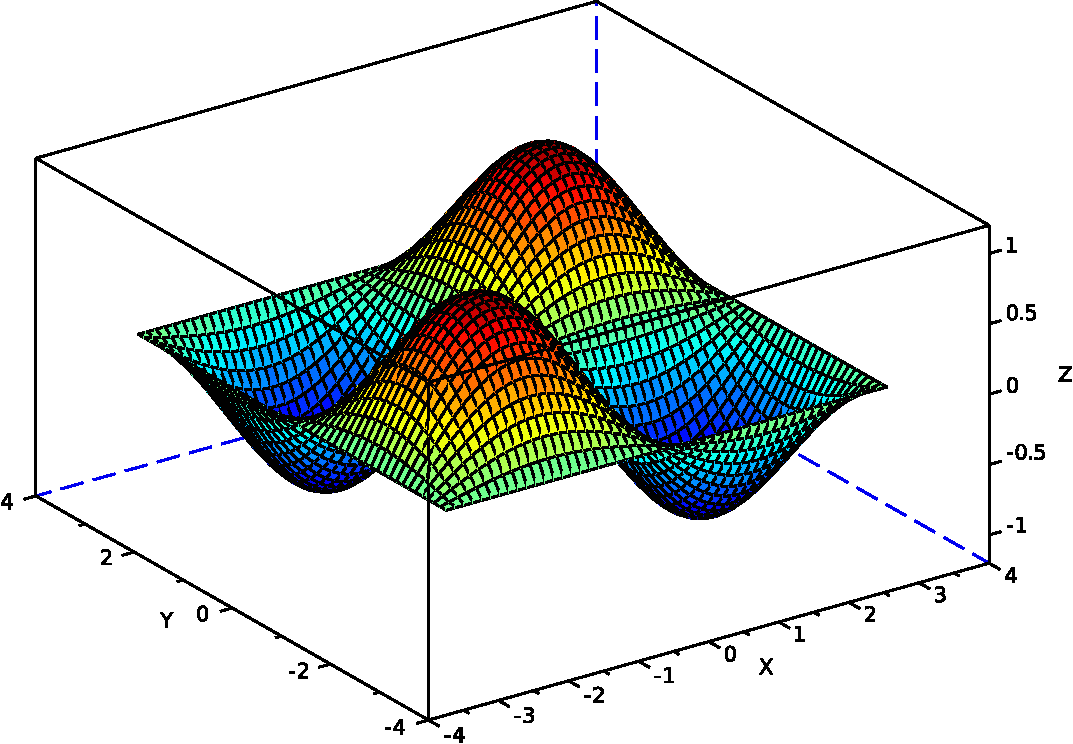
\includegraphics[scale=0.5]{poisson2d.pdf}
\par
\caption{Solusi persamaan Laplace $u(x,y)$}
\end{figure}


\section{Persamaan transfer kalor}

Hitung solusi numerik dari
\begin{equation}
\frac{\partial^2 u(x,t)}{\partial x^2} = \frac{\partial u(x,t)}{\partial t}
\end{equation}
untuk $0 \leq x \leq 1$ dan $0 \leq t \leq 0.1$ dengan syarat awal
\begin{equation}
u(x,0) = \sin(\pi x)
\end{equation}
dan syarat batas
\begin{equation}
u(0,t) = 0,\hspace{0.5cm} u(1,t) = 0
\end{equation}
Gunakan metode Euler eksplisit, Euler implisit dan Crank-Nicolson serta
bandingkan hasilnya.
Buat juga animasi (dalam format GIF) yang menggambarkan perubatan profil
suhu terhadap waktu.

\section{Persamaan gelombang}

Selesaikan PDE berikut dengan menggunakan metode beda hingga.
Buat juga visualisasi solusi berupa animasi dari solusi yang didapatkan.

\begin{enumerate}[label=(\alph*)]
%
\item Hitung solusi numerik persamaan gelombang 1d
\begin{equation}
\frac{\partial^2 u(x,t)}{\partial x^2} = \frac{\partial^2 u(x,t)}{\partial t^2}
\end{equation}
untuk $0 < x < 1$ dan $0 \leq t \leq 5$ dengan syarat awal
\begin{align*}
u(x,0)  & = \sin\left(2\pi x\right) \\
u'(x,0) & = 0
\end{align*}
dan syarat batas:
\begin{equation*}
u(0,t) = 0, \hspace{0.5cm} u(1,t) = 0
\end{equation*}
%
\item Selesaikan persamaan gelombang 2d
\begin{equation}
\frac{1}{4}\left(\frac{\partial^2 u(x,y,t)}{\partial x^2} +
\frac{\partial^2 u(x,y,t)}{\partial y^2}\right)
= \frac{\partial^2 u(x,y,t)}{\partial t^2}
\end{equation}
pada domain rektangular dengan $0 < x < 1$ dan $0 < y < 1$ serta
pada selang waktu $0 < t < 2$ dengan syarat awal
\begin{equation*}
u(x,y,0) = \sin(6\pi x)\sin(2\pi y)
\end{equation*}
dan syarat batas:
\begin{align*}
u(0,y,t) = 0, \hspace{0.5cm} u(x,0,t) = 0 \\
u(1,y,t) = 0, \hspace{0.5cm} u(x,1,t) = 0
\end{align*}

\begin{figure}[H]
\centering
\includegraphics[scale=0.5]{images/TEMP_wave2d_0000.pdf}
\par
\caption{Syarat awal $u(x,y,0)$}
\end{figure}
%
\end{enumerate}


%\textbf{SOLUSI}

Dengan menggunakan notasi berikut:
\begin{equation}
y_1 \equiv y, \hspace{1cm} y_2 \equiv y'
\end{equation}

%\begin{mdframed}[backgroundcolor=mintedbg]
%\inputminted[breaklines]{scilab}{soal_01.sce}
%\end{mdframed}


\begin{figure}[H]
\centering
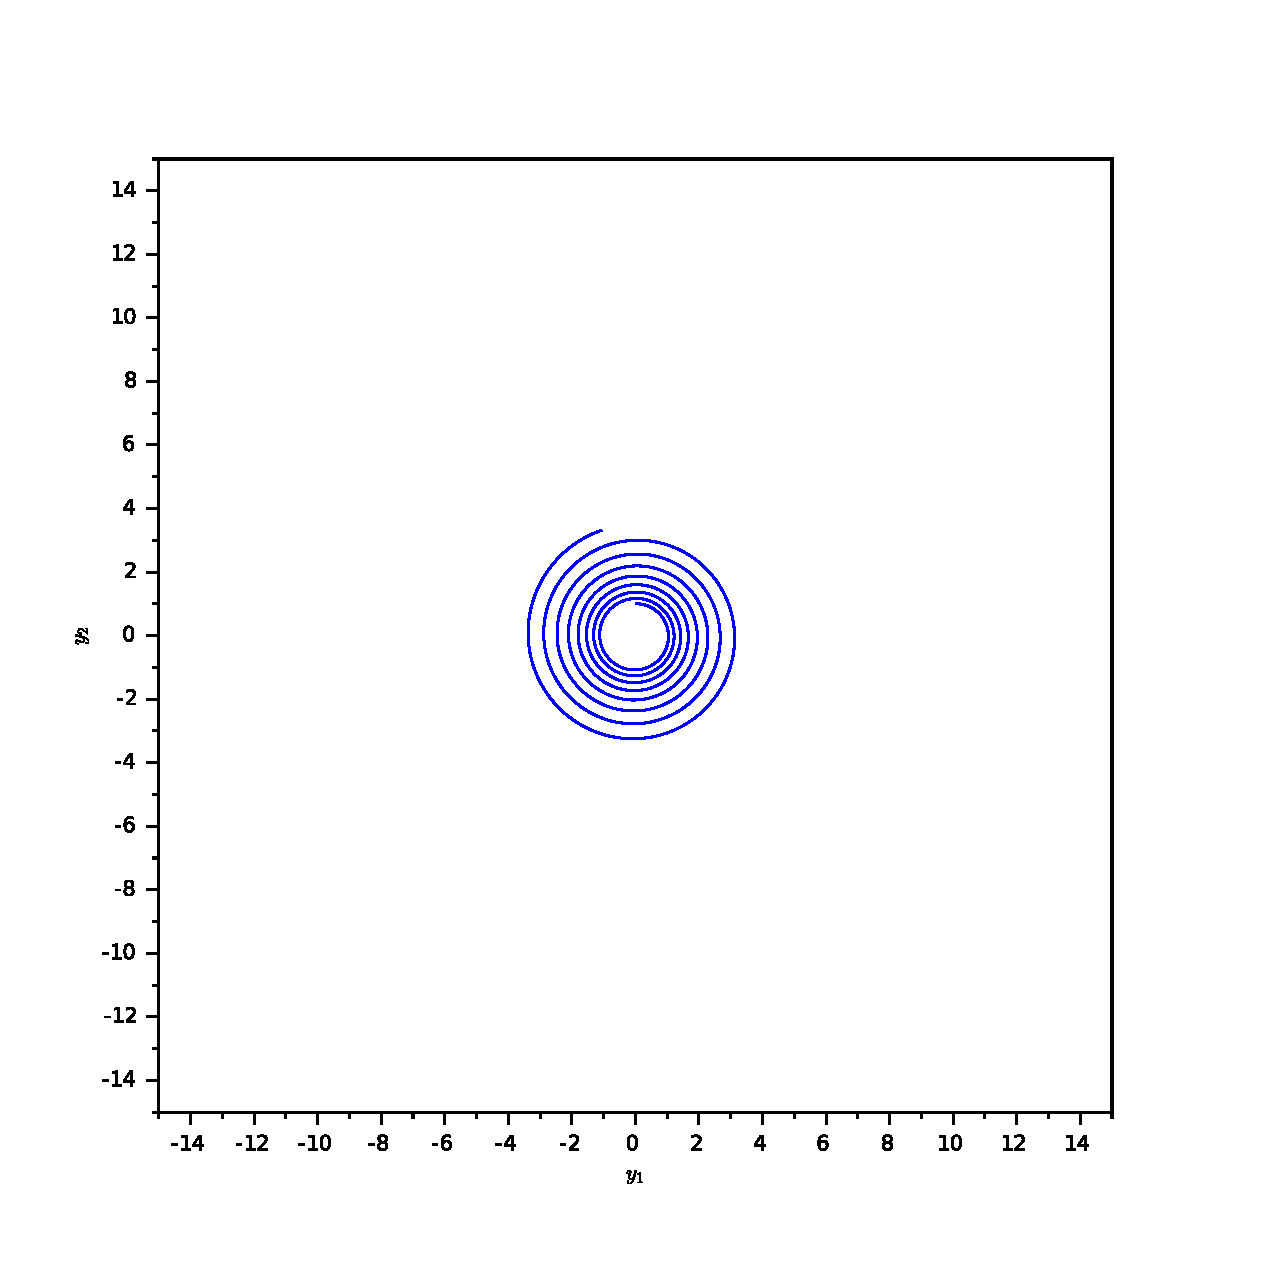
\includegraphics[width=0.3\textwidth]{images/soal_01_ode_euler_y1_y2.pdf}
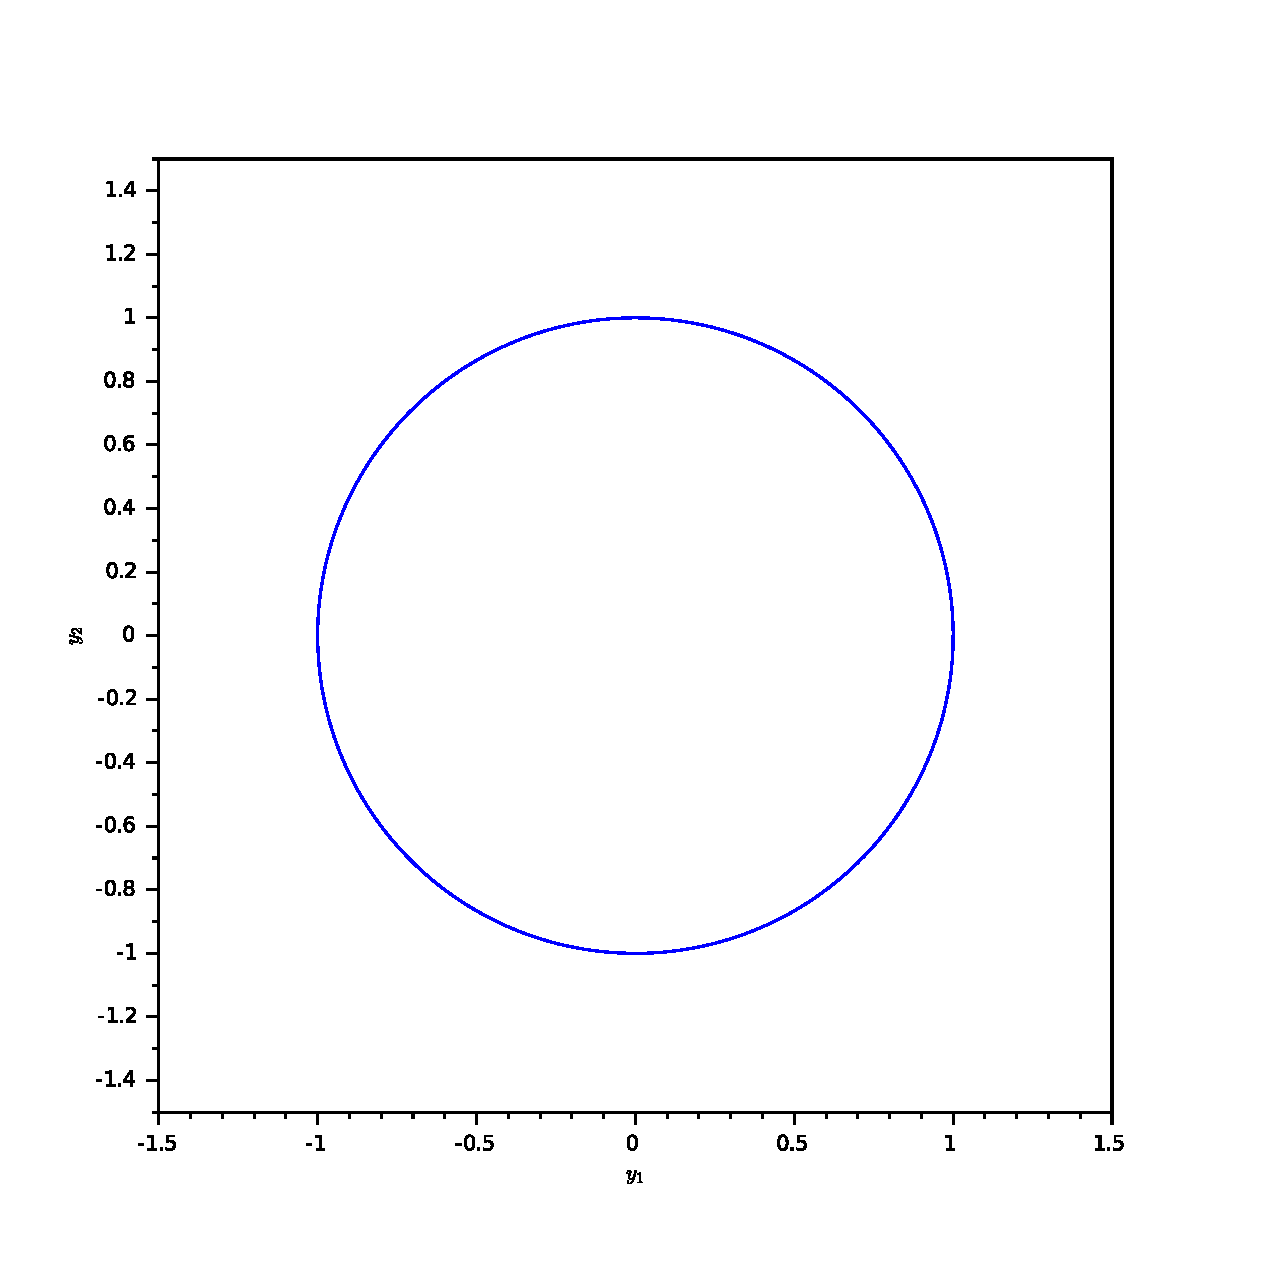
\includegraphics[width=0.3\textwidth]{images/soal_01_ode_euler_PC_y1_y2.pdf}
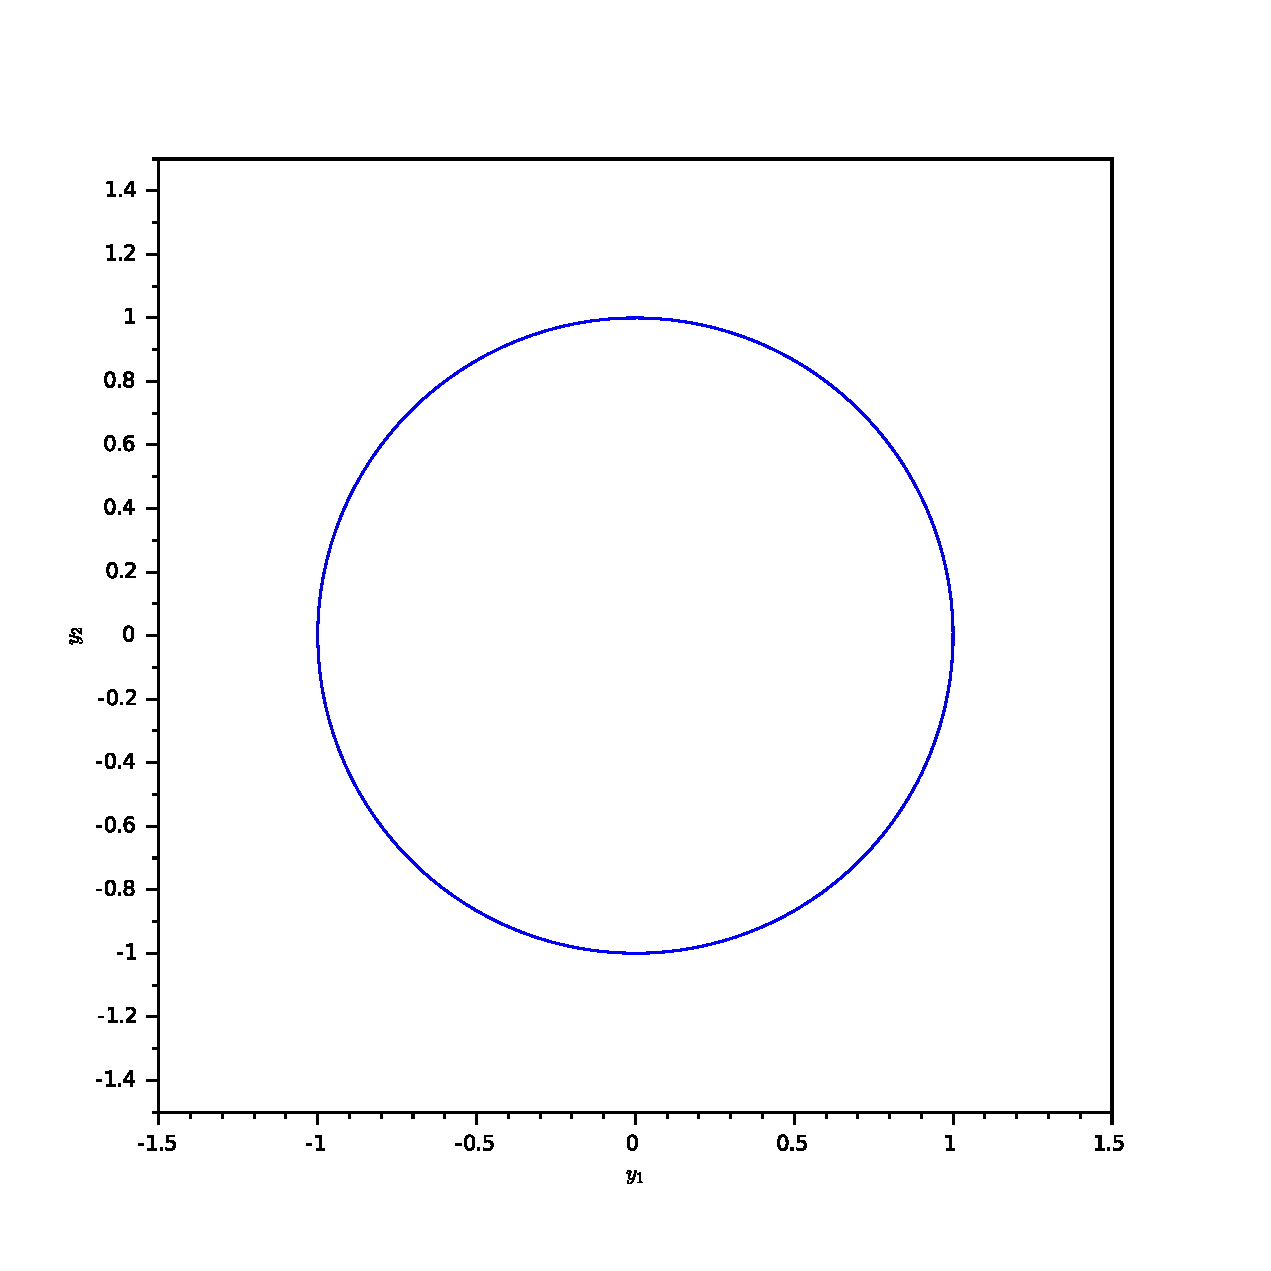
\includegraphics[width=0.3\textwidth]{images/soal_01_ode_RK4_y1_y2.pdf}
\par
\end{figure}

\begin{figure}[H]
\centering
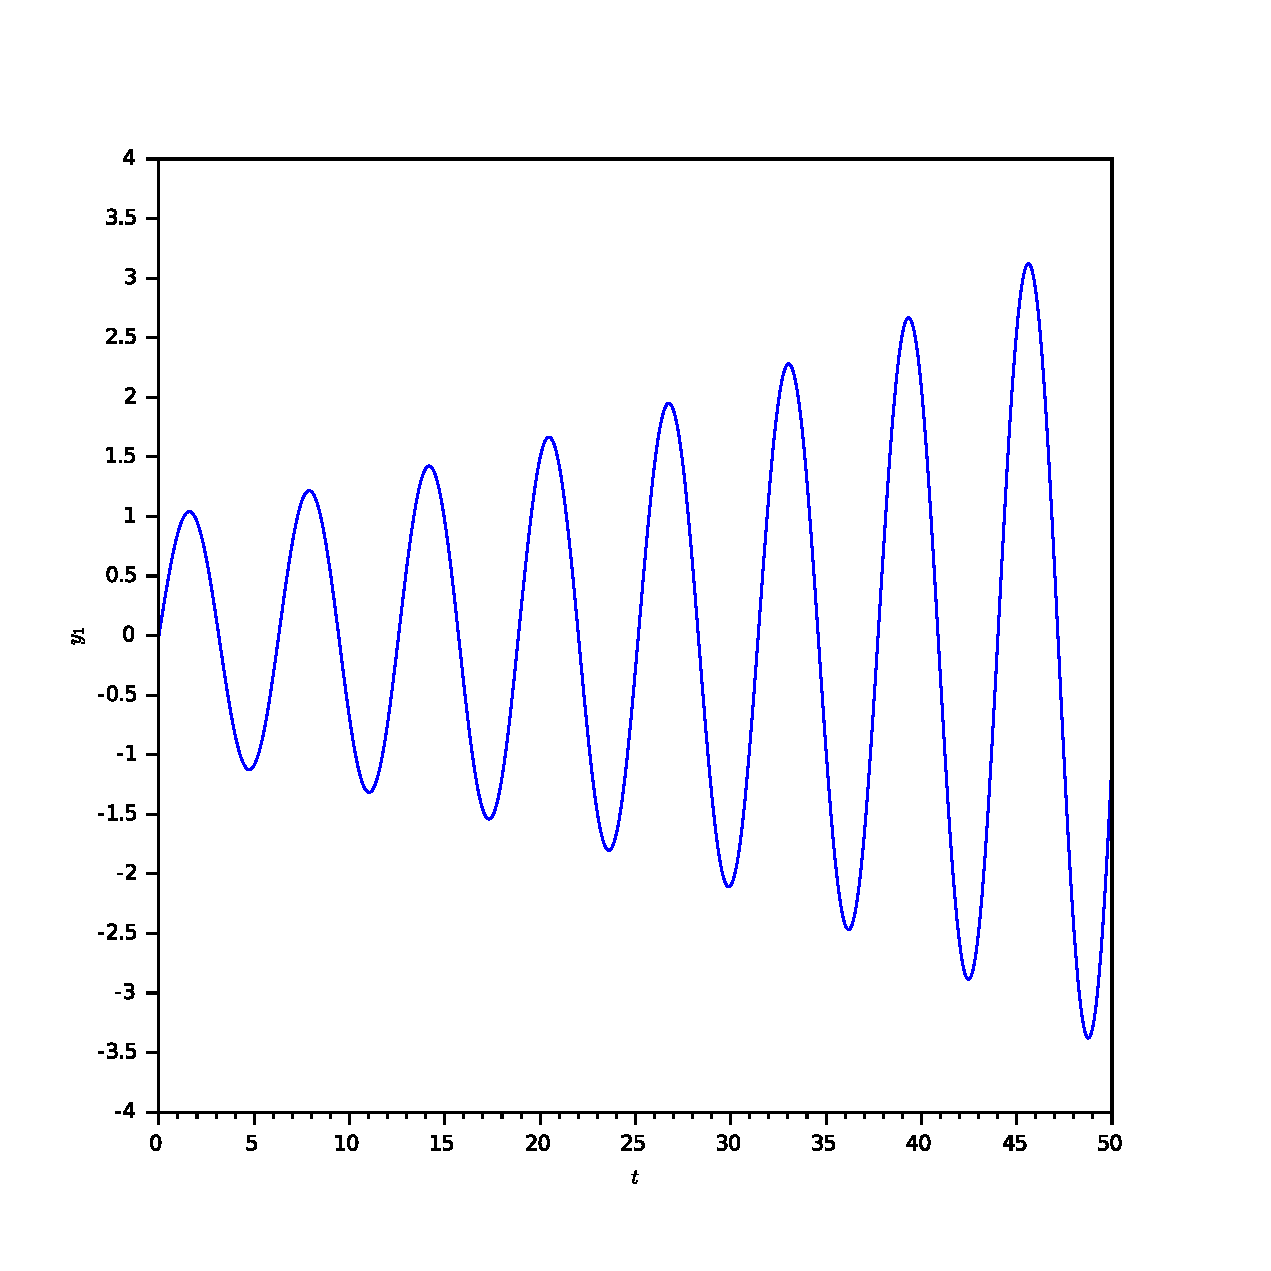
\includegraphics[width=0.3\textwidth]{images/soal_01_ode_euler_t_y1.pdf}
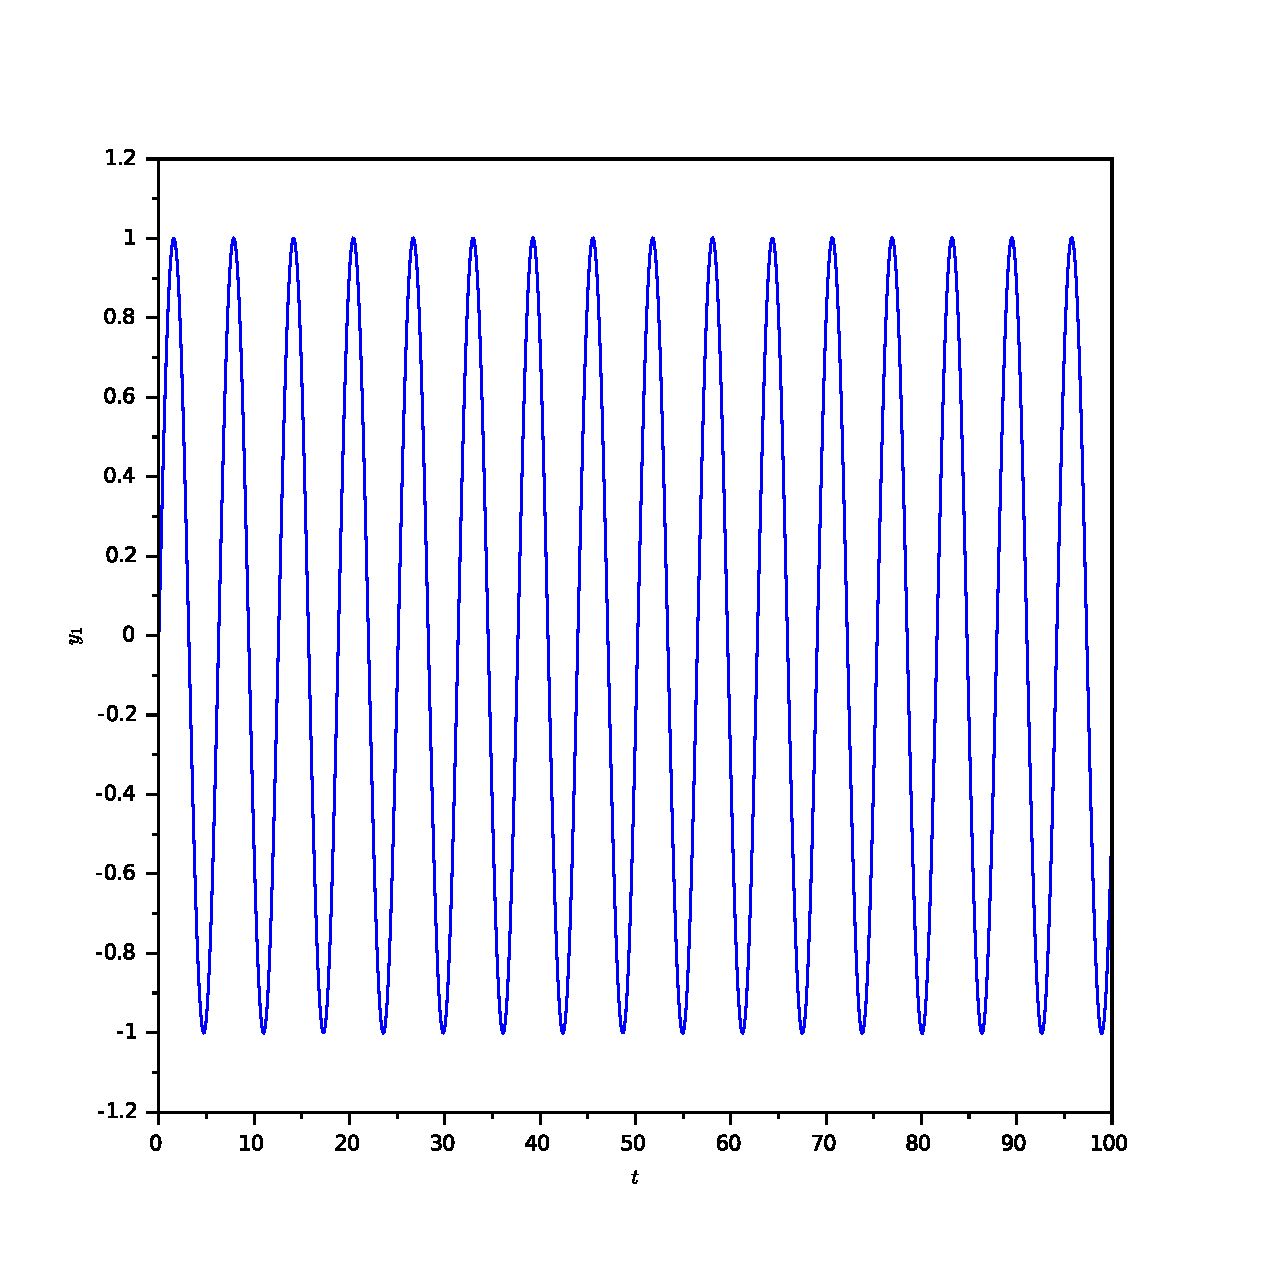
\includegraphics[width=0.3\textwidth]{images/soal_01_ode_euler_PC_t_y1.pdf}
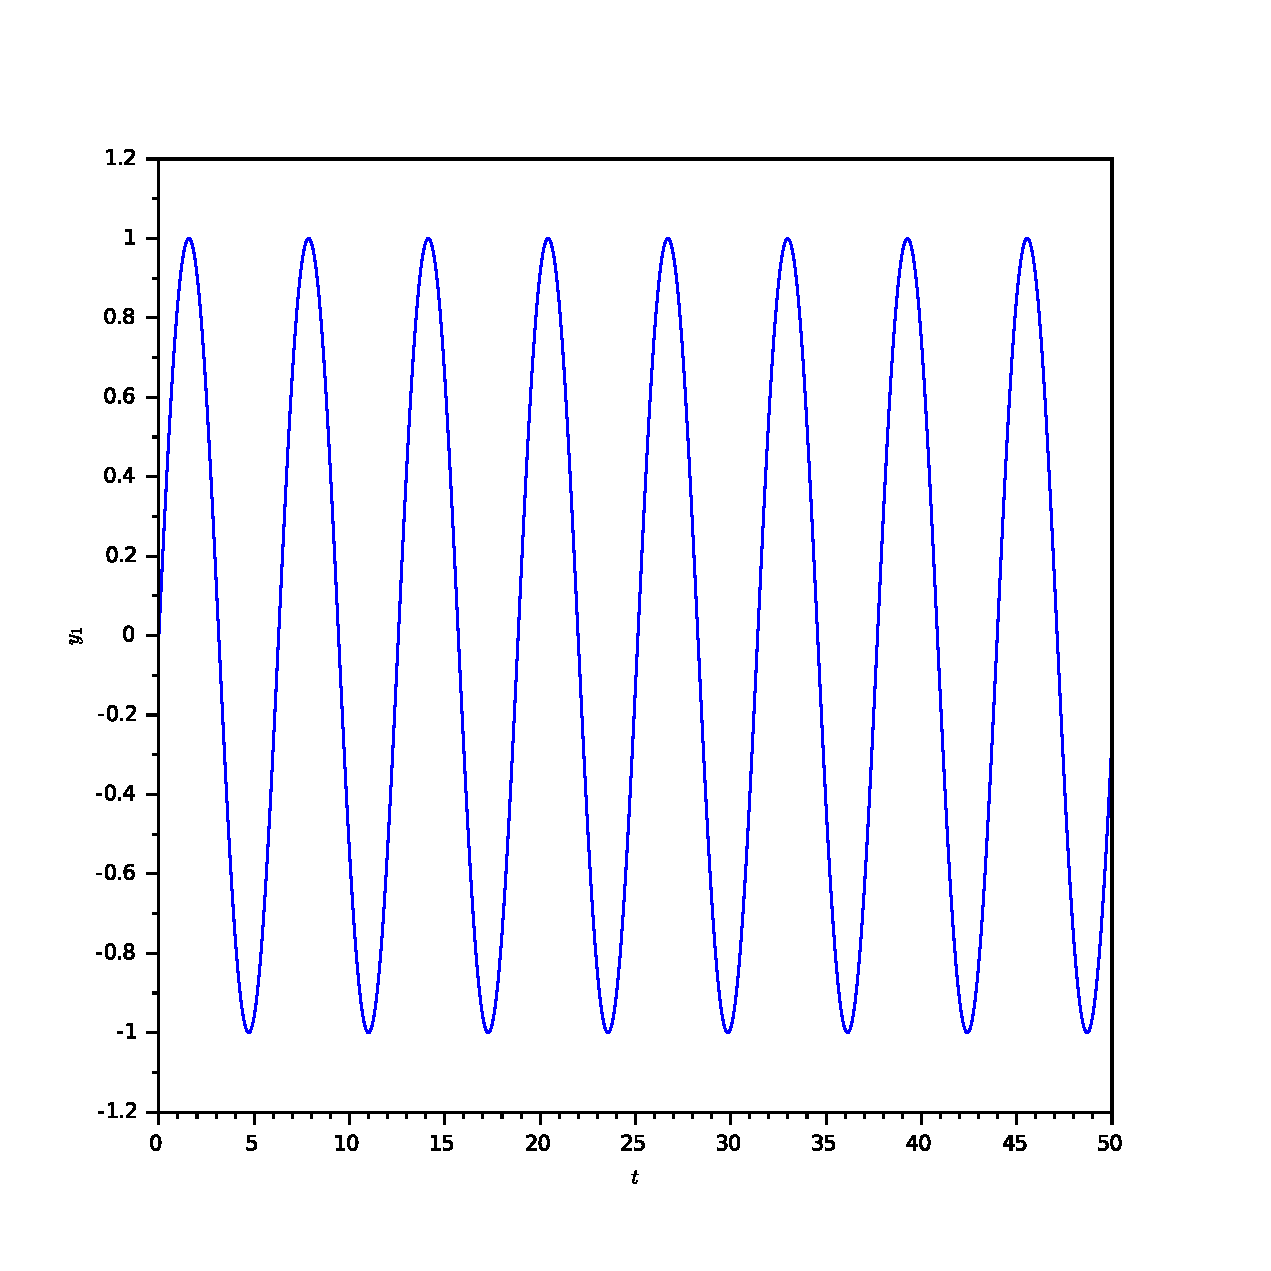
\includegraphics[width=0.3\textwidth]{images/soal_01_ode_RK4_t_y1.pdf}
\par
\end{figure}
%\section{Soal 2: Gerakan pendulum}

Gerakan pendulum
%\section{Soal 3: metode shooting}

soal a

soal b

Metode shooting untuk quantum harmonic oscillator

%\section{Soal 4: Persamaan Schrodinger melalui eigenvalue}

(a) harmonic oscillator
%\section{Soal 5: Persamaan Poisson 2D}
%\section{Soal 6: difusi dan kalor}
%\section{Soal 7: Persamaan gelombang}

\end{document}
